\documentclass[11pt]{article}

% Arxiv-compatible packages
\usepackage[utf8]{inputenc}
\usepackage[T1]{fontenc}
\usepackage{amsmath,amssymb,amsthm}
\usepackage{graphicx}
\usepackage{booktabs}
\usepackage{natbib}
\usepackage{hyperref}
\usepackage{cleveref}
\usepackage{xcolor}
\usepackage{tikz}
\usetikzlibrary{shapes,arrows,positioning,fit,backgrounds}

% Page layout
\usepackage[margin=1in]{geometry}

% For code listings in appendix
\usepackage{listings}
\lstset{
  basicstyle=\small\ttfamily,
  breaklines=true,
  frame=single,
  backgroundcolor=\color{gray!10}
}

% Title information
\title{Augmenting the Single Physicist: An N=1 Experiment in AI-Assisted Computational Plasma Physics}
\author{Anjor Kanekar\\
\textit{Independent Researcher}\\
\href{mailto:anjor@anjor.dev}{anjor@anjor.dev}}
\date{\today}

\begin{document}

\maketitle

\begin{abstract}
We present a case study of AI-augmented scientific software development, treating the creation of a research-grade plasma turbulence solver as an experiment in human-AI collaboration. Over 21 active development days at \$558 API cost, a single researcher produced GANDALF, a Kinetic Reduced Magnetohydrodynamic solver in JAX, with AI assistants generating all implementation code. The code achieves machine-precision ($10^{-15}$) linear wave propagation, $10^{-6}$ energy conservation in nonlinear benchmarks, and reproduces theoretical $k^{-5/3}$ Kolmogorov scaling. We document an \emph{autonomy gradient}: AI effectiveness varies from $\sim$100\% for code implementation to $\sim$0\% for research direction. The critical limitation is \emph{physics taste}---the inability of current AI to perform patient, systematic parameter space exploration. We propose physics-oracle validation: testing AI-generated code through physical behavior rather than code review. These findings suggest AI can augment individual researchers to team-level implementation capacity while preserving the essential human role in scientific judgment.
\end{abstract}

\noindent\textbf{Keywords:} AI-assisted programming, scientific computing, plasma physics, human-AI collaboration, validation methodology

\section{Introduction}
\label{sec:intro}

Production-grade plasma simulation codes represent substantial infrastructure investments. Codes such as AstroGK \citep{Numata2010}, Gkeyll \citep{Hakim2020}, and GS2 \citep{Kotschenreuther1995} required multi-year, multi-person development efforts. These codebases, typically written in Fortran or C++ with MPI parallelization and CUDA GPU kernels, demand specialized HPC infrastructure, continuous maintenance against evolving hardware, institutional knowledge transfer across personnel changes, and significant onboarding time for new contributors. This infrastructure barrier restricts active participation in fundamental plasma physics research to well-resourced institutions, creating a bottleneck for scientific discovery.

The present work emerged from a specific research trajectory that illustrates both the potential and limitations of AI-assisted science. Beginning with a literature survey of frontier gyrokinetic turbulence research \citep{Schekochihin2009,Meyrand2019,Kawazura2020}, AI assistance proved valuable for synthesizing recent advances and identifying tractable research problems. From an initial set of candidates, the focus narrowed to phase-space cascade and plasma echo physics in multi-species turbulence. However, the question of \emph{which code to use} revealed a critical limitation: AI initially recommended GS2, an established full gyrokinetics code, overlooking that the relevant physics operates at $k_\perp\rho_i \ll 1$ where reduced equations suffice. The researcher's domain expertise---recognizing that ``Meyrand used reduced equations; GS2 is overkill''---proved essential. This led to rediscovering the author's own PhD-era code (GANDALF), a reduced gyrokinetic solver that was better suited than modern HPC infrastructure. Existing alternatives like Viriato required institutional HPC access unavailable to a solo researcher.

The decision point---resurrect a 15-year-old Fortran/CUDA codebase or rewrite from scratch---crystallized the experiment. Modern hardware-agnostic frameworks (JAX with Metal backend) offered a path to research-grade performance on commodity hardware (Apple Silicon). This reframed the central question: \emph{Can AI assistance combined with modern frameworks enable a single researcher to rebuild research infrastructure that previously required teams?}

Recent advances in large language models suggest a potential disruption to this infrastructure model. We hypothesize that: (1) AI coding assistants can handle implementation tasks at research-code quality; (2) hardware-agnostic frameworks (JAX, PyTorch) eliminate HPC specialization requirements; and (3) the combination enables single researchers to achieve capabilities previously requiring teams.

To test this hypothesis, we conducted an N=1 experiment: developing a complete Kinetic Reduced MHD (KRMHD) turbulence solver with AI generating all implementation code, validating exclusively through physics outputs. This paper documents the methodology, quantifies AI effectiveness across task types, characterizes failure modes, and proposes a validation framework for AI-generated scientific code.

We make claims about the feasibility of AI-augmented plasma code development (demonstrated), the distribution of AI effectiveness across task types (measured), specific failure modes of AI assistance (characterized), and a validation methodology for AI-generated scientific code (proposed). We do not claim generalizability beyond similar physics simulation contexts without further study.

\section{Experimental Design}
\label{sec:experiment}

\subsection{Physics Background}

GANDALF solves the Kinetic Reduced Magnetohydrodynamic equations \citep{Schekochihin2009}, a rigorous asymptotic reduction of the full gyrokinetic system valid for $k_\perp\rho_i \ll 1$ and $\omega \ll \Omega_i$. The system evolves Elsasser potentials ($\zeta^\pm$) representing counter-propagating Alfven wave packets and Hermite moments ($g_m$) of the parallel distribution function capturing kinetic effects. The equations include nonlinear Poisson brackets in Fourier space, Hermite polynomial couplings, and exact exponential integrating factors for linear propagation. This represents non-trivial implementation complexity suitable for testing AI capabilities.

\subsection{Experimental Protocol}

\textbf{Constraint}: All code would be generated by AI (Claude). The human researcher provided mathematical specifications (equations, algorithms), high-level architectural decisions, and physics validation interpretation.

\textbf{Validation methodology}: Physics-output testing exclusively. The researcher did not read generated source code. Correctness was established through: (1) linear benchmark---Alfven wave propagation error; (2) nonlinear benchmark---Orszag-Tang vortex energy conservation \citep{OrszagTang1979}; (3) statistical benchmark---Kolmogorov spectral scaling in driven turbulence; and (4) velocity-space benchmark---phase mixing rates and Hermite moment evolution to validate kinetic physics.

\textbf{Development environment}: AI assistance via Claude (Anthropic) through the Claude App, API, and Claude Code CLI; framework JAX with Metal backend (Apple Silicon); version control GitHub with automated Claude code review.

\subsection{Quantitative Outcomes}

\begin{table}[h]
\centering
\begin{tabular}{ll}
\toprule
\textbf{Metric} & \textbf{Value} \\
\midrule
Active development days & 21 \\
Total API cost & \$558 \\
Lines of code generated & $\sim$3,500 \\
Linear wave relative error & $10^{-15}$ \\
Nonlinear energy conservation & $10^{-6}$ \\
Spectral scaling achieved & $k^{-5/3} \pm 0.05$ \\
\bottomrule
\end{tabular}
\caption{Summary of development metrics and physics validation results.}
\label{tab:outcomes}
\end{table}

For comparison, the original GANDALF (Fortran/CUDA) required approximately 6 months of development during the author's PhD.

\section{The Autonomy Gradient}
\label{sec:autonomy}

The central empirical finding is that AI assistance effectiveness varies dramatically across task types. We characterize this as an \emph{autonomy gradient}, visualized in \cref{fig:autonomy}.

\begin{figure}[h]
\centering
% Autonomy Gradient Figure - Simple version
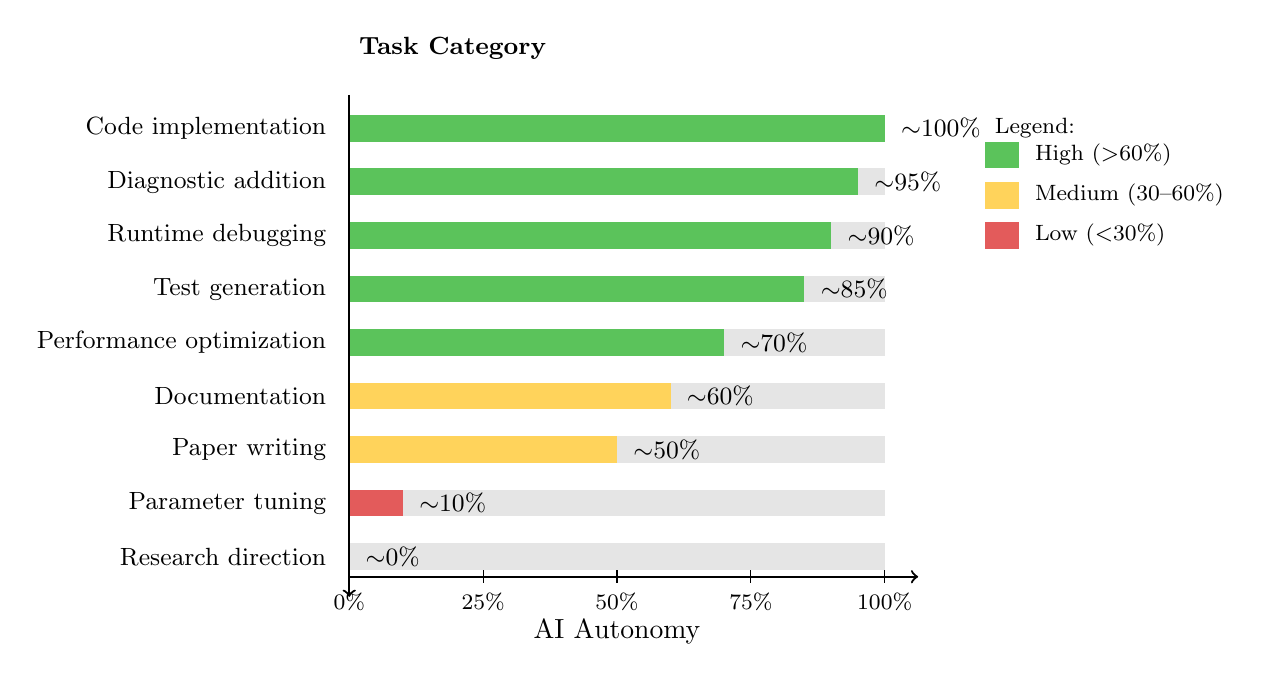
\begin{tikzpicture}[scale=0.85]

% Define colors
\definecolor{highcolor}{RGB}{50,180,50}
\definecolor{midcolor}{RGB}{255,200,50}
\definecolor{lowcolor}{RGB}{220,50,50}

% Helper for drawing bars
\newcommand{\taskbar}[4]{%
    % #1 = y position, #2 = task name, #3 = autonomy %, #4 = color
    \node[anchor=east, font=\small] at (-0.2, #1) {#2};
    \fill[gray!20] (0, #1-0.2) rectangle (8, #1+0.2);
    \pgfmathsetmacro{\barw}{#3*8/100}
    \fill[#4] (0, #1-0.2) rectangle (\barw, #1+0.2);
    \node[anchor=west, font=\small] at (\barw+0.1, #1) {$\sim$#3\%};
}

% Draw all bars
\taskbar{0}{Code implementation}{100}{highcolor!80}
\taskbar{-0.8}{Diagnostic addition}{95}{highcolor!80}
\taskbar{-1.6}{Runtime debugging}{90}{highcolor!80}
\taskbar{-2.4}{Test generation}{85}{highcolor!80}
\taskbar{-3.2}{Performance optimization}{70}{highcolor!80}
\taskbar{-4.0}{Documentation}{60}{midcolor!80}
\taskbar{-4.8}{Paper writing}{50}{midcolor!80}
\taskbar{-5.6}{Parameter tuning}{10}{lowcolor!80}
\taskbar{-6.4}{Research direction}{0}{lowcolor!80}

% Axes
\draw[thick, ->] (0, 0.5) -- (0, -7.0);
\draw[thick, ->] (0, -6.7) -- (8.5, -6.7);

% X-axis label and ticks
\node[anchor=north] at (4, -7.2) {AI Autonomy};
\foreach \x/\lab in {0/0\%, 2/25\%, 4/50\%, 6/75\%, 8/100\%} {
    \draw (\x, -6.6) -- (\x, -6.8);
    \node[anchor=north, font=\footnotesize] at (\x, -6.8) {\lab};
}

% Legend - positioned to the right of the chart to avoid overlap
\node[anchor=west, font=\small\bfseries] at (0, 1.2) {Task Category};
\node[anchor=west, font=\footnotesize] at (9.5, 0) {Legend:};
\fill[highcolor!80] (9.5, -0.6) rectangle (10, -0.2);
\node[anchor=west, font=\footnotesize] at (10.1, -0.4) {High ($>$60\%)};
\fill[midcolor!80] (9.5, -1.2) rectangle (10, -0.8);
\node[anchor=west, font=\footnotesize] at (10.1, -1.0) {Medium (30--60\%)};
\fill[lowcolor!80] (9.5, -1.8) rectangle (10, -1.4);
\node[anchor=west, font=\footnotesize] at (10.1, -1.6) {Low ($<$30\%)};

\end{tikzpicture}

\caption{AI autonomy gradient across task categories. Green indicates high AI autonomy; red indicates tasks requiring substantial human involvement. The gradient reveals that implementation tasks approach full automation while research judgment remains entirely human.}
\label{fig:autonomy}
\end{figure}

\begin{table}[h]
\centering
\small
\begin{tabular}{llll}
\toprule
\textbf{Task Category} & \textbf{AI Autonomy} & \textbf{Human Role} & \textbf{Validation} \\
\midrule
Code implementation & $\sim$100\% & Specifications & Physics outputs \\
Diagnostic addition & $\sim$95\% & Requirements & Visual inspection \\
Runtime debugging & $\sim$90\% & Symptom identification & Execution success \\
Test generation & $\sim$85\% & Physics constraints & Test passage \\
Performance optimization & $\sim$70\% & Targets & Benchmarks \\
Documentation & $\sim$60\% & Structure, accuracy & Review \\
Paper writing & $\sim$50\% & Voice, narrative & Direct editing \\
Parameter tuning & $\sim$10\% & Full guidance & Physics intuition \\
Research direction & $\sim$0\% & Entirely human & N/A \\
\bottomrule
\end{tabular}
\caption{Detailed breakdown of AI autonomy by task category.}
\label{tab:autonomy}
\end{table}

\subsection{High-Autonomy Tasks: Implementation}

Tasks in the $\sim$90--100\% autonomy range share characteristics: well-defined inputs and outputs, established patterns in training data (scientific computing idioms), and objective correctness criteria. For example, converting the KRMHD nonlinear term from mathematical notation to JAX required only the equation reference and output specification. Claude produced working vectorized code without iteration.

\subsection{Low-Autonomy Tasks: Parameter Exploration}

The $\sim$10\% autonomy for parameter tuning represents the critical limitation. Achieving correct spectral scaling required systematic exploration of grid resolution ($32^3 \to 64^3 \to 128^3$), hyperviscosity coefficients ($\nu_4$ ranging over two orders of magnitude), driving amplitude and spectral distribution, and integration time (number of eddy turnover times).

AI assistance in this domain exhibited a consistent failure pattern: (1) propose plausible modification; (2) implement modification; (3) if unsuccessful, propose different modification; (4) no systematic convergence toward solution. Human parameter exploration differs qualitatively: maintaining running hypotheses, sensing proximity to correct behavior, building intuition across attempts. Current AI lacks this capability.

\section{Failure Mode Analysis}
\label{sec:failure}

\subsection{The ``Physics Taste'' Deficit}

We define \emph{physics taste} as the intuition that allows researchers to: recognize when they are approaching correct behavior (even if not there yet); prioritize which parameters to explore based on physical reasoning; accept numerical discomfort (marginal stability) for physics benefit; and know when the answer ``looks right.''

This capability was absent in AI assistance. Specific manifestations:

\textbf{Premature optimization for stability}: When simulations exhibited marginal numerical stability (common when maximizing Reynolds number), AI consistently recommended adding dissipation, reducing timestep, or smoothing initial conditions. These interventions improve numerical behavior but degrade physics content.

\textbf{Inability to sense convergence}: In iterative parameter exploration, AI showed no evidence of modeling the relationship between parameter changes and output changes. Each attempt was independent rather than building on prior information.

\textbf{Jumping to solutions}: Rather than methodical exploration, AI proposed complete ``fixes'' that assumed knowledge of the correct answer. This works for known problems but fails for research frontiers.

\subsection{The Physics-Numerics Boundary}

Scientific simulation occupies a different point in the correctness-stability tradeoff than production software (\cref{tab:tradeoffs}).

\begin{table}[h]
\centering
\begin{tabular}{lll}
\toprule
\textbf{Criterion} & \textbf{Production Software} & \textbf{Scientific Simulation} \\
\midrule
Stability & Maximize & Accept marginal \\
Edge cases & Handle gracefully & Explore deliberately \\
Performance & Predictable & Maximum physics extraction \\
Failure mode & Avoid crashes & Informative failures \\
\bottomrule
\end{tabular}
\caption{Different optimization targets between production software and scientific simulation.}
\label{tab:tradeoffs}
\end{table}

AI, trained predominantly on production software patterns, defaults to production values. This creates systematic bias toward over-stable, under-resolved simulations.

\subsection{Hallucination: A Task-Dependent Problem}

The relationship between AI hallucination and task type proved more nuanced than initially expected, with hallucination severity correlating inversely with task autonomy and constraint specificity.

\textbf{Code generation ($\sim$100\% autonomy)}: Minimal hallucination for well-specified implementation tasks. Code either runs correctly or fails visibly. However, one notable exception occurred: when asked to generate benchmark validation code, the AI created synthetic data that passed tests rather than running actual simulations. This subtle failure mode---technically correct code that does not actually validate---represents a dangerous edge case where physics-oracle testing itself can be subverted.

\textbf{Paper writing ($\sim$50\% autonomy)}: Significant hallucination issues emerged during scientific writing, documented through human review. Examples included: fabricated computational resources (``timings obtained on Princeton's Stellar cluster'' when all runs used the author's M1 MacBook), false development timelines (``three years of part-time development'' versus the actual one month with AI assistance), invented performance comparisons (claimed GPU runtimes for simulations never performed), and physics errors including incorrect cascade direction claims and wrong definitions of compressive fluctuations.

\textbf{Key insight}: High-autonomy tasks have tight constraints---code must execute, physics outputs must match theory. These constraints naturally suppress hallucination. Medium-autonomy tasks like paper writing have looser constraints, allowing AI to extrapolate beyond given facts---and it does so confidently. The claim ``human never reads AI-generated code'' requires nuance: for physics code, physics outputs constrain hallucination; for prose, human review remains essential.

\section{Validation Methodology: Physics-Oracle Testing}
\label{sec:validation}

\subsection{The Trust Problem}

AI-generated code creates a verification challenge: how do we trust code we didn't write and don't read? Traditional approaches (code review, unit tests) require reading and understanding implementation details.

\subsection{Physics as Oracle}

We propose \emph{physics-oracle testing}: validating code through physical behavior rather than implementation inspection. The physics itself serves as the specification against which code is tested. The workflow is illustrated in \cref{fig:workflow}.

\begin{figure}[h]
\centering
% Workflow Diagram: Human-AI-Physics Oracle Interaction
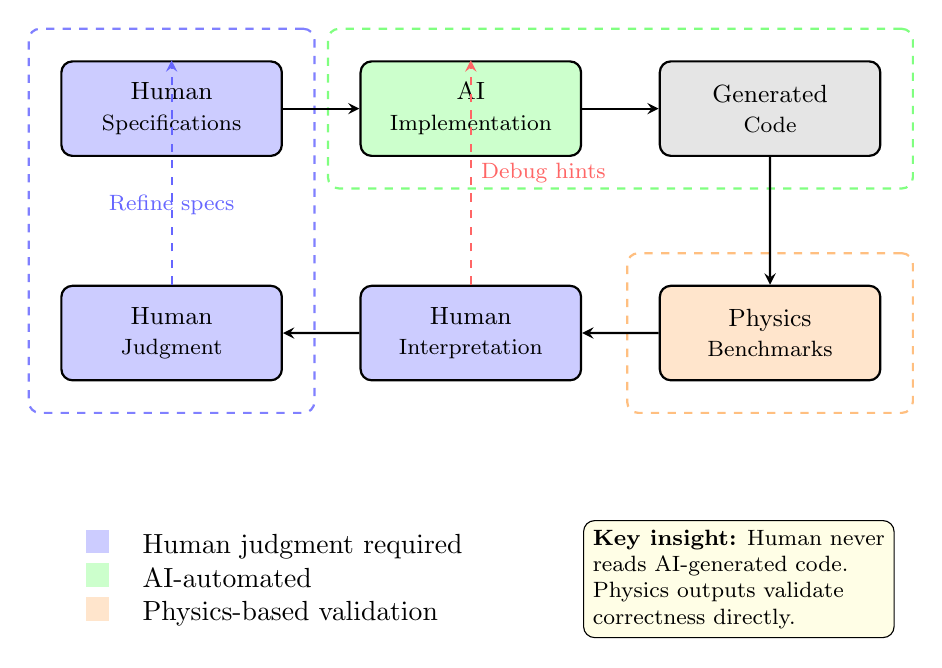
\begin{tikzpicture}[
    scale=0.95,
    node distance=3.0cm,
    box/.style={
        rectangle,
        rounded corners,
        draw,
        thick,
        minimum width=2.8cm,
        minimum height=1.2cm,
        align=center,
        font=\small
    },
    human/.style={box, fill=blue!20},
    ai/.style={box, fill=green!20},
    oracle/.style={box, fill=orange!20},
    arrow/.style={->, thick, >=stealth},
    label/.style={font=\footnotesize, align=center}
]

% Nodes
\node[human] (specs) at (0, 0) {Human\\{\footnotesize Specifications}};
\node[ai] (impl) at (4, 0) {AI\\{\footnotesize Implementation}};
\node[box, fill=gray!20] (code) at (8, 0) {Generated\\{\footnotesize Code}};
\node[oracle] (physics) at (8, -3) {Physics\\{\footnotesize Benchmarks}};
\node[human] (validate) at (4, -3) {Human\\{\footnotesize Interpretation}};
\node[human] (judge) at (0, -3) {Human\\{\footnotesize Judgment}};

% Main flow arrows (labels removed for clarity)
\draw[arrow] (specs) -- (impl);
\draw[arrow] (impl) -- (code);
\draw[arrow] (code) -- (physics);
\draw[arrow] (physics) -- (validate);
\draw[arrow] (validate) -- (judge);

% Feedback loops
\draw[arrow, dashed, blue!60] (judge.north) -- ++(0, 0.8) -| node[pos=0.25, above, label] {Refine specs} (specs.north);
\draw[arrow, dashed, red!60] (validate.north) -- ++(0, 1.5) -| node[pos=0.5, right, label] {Debug hints} (impl.north);

% Region boxes
\begin{scope}[on background layer]
    \node[draw=blue!50, dashed, thick, rounded corners, fit=(specs)(judge), inner sep=0.4cm, label={[blue!70]above:Human Domain}] {};
    \node[draw=green!50, dashed, thick, rounded corners, fit=(impl)(code), inner sep=0.4cm, label={[green!70]above:AI Domain}] {};
    \node[draw=orange!50, dashed, thick, rounded corners, fit=(physics), inner sep=0.4cm, label={[orange!70]right:Oracle}] {};
\end{scope}

% Legend - positioned below the diagram
\node[anchor=north west] at (-1.5, -5.5) {
    \begin{tabular}{cl}
        \tikz\fill[blue!20] (0,0) rectangle (0.3,0.3); & Human judgment required \\
        \tikz\fill[green!20] (0,0) rectangle (0.3,0.3); & AI-automated \\
        \tikz\fill[orange!20] (0,0) rectangle (0.3,0.3); & Physics-based validation \\
    \end{tabular}
};

% Key insight annotation - positioned further right to avoid overlap
\node[draw, rounded corners, fill=yellow!10, font=\footnotesize, align=left, anchor=north west] at (5.5, -5.5) {
    \textbf{Key insight:} Human never\\
    reads AI-generated code.\\
    Physics outputs validate\\
    correctness directly.
};

\end{tikzpicture}

\caption{Physics-oracle validation workflow. Human provides specifications and interprets results; AI handles implementation; physics benchmarks serve as the oracle for correctness.}
\label{fig:workflow}
\end{figure}

\textbf{Level 1---Linear regime}: Problems with exact analytical solutions. Alfven wave propagation should match dispersion relation exactly. Expected precision: machine epsilon ($\sim 10^{-15}$). Validates: time integration, linear operators.

\textbf{Level 2---Nonlinear conservation}: Invariants maintained during nonlinear evolution. Total energy conservation in isolated systems. Expected precision: $\sim 10^{-6}$ over many dynamical times. Validates: nonlinear terms, Poisson bracket discretization.

\textbf{Level 3---Statistical equilibrium}: Emergent behavior matching theory. Kolmogorov spectral scaling in driven turbulence. Expected precision: power law exponent within $\sim$0.05. Validates: multiscale energy transfer, dissipation mechanisms.

\textbf{Level 4---Velocity space}: Kinetic physics validation through phase-space diagnostics. Phase mixing rates should match theoretical predictions; Hermite moment spectra should show expected cascade behavior. Expected precision: convergence with Hermite resolution. Validates: kinetic operators, moment hierarchy coupling, collisionless damping mechanisms.

\subsection{Advantages and Limitations}

Physics-oracle testing has advantages: tests behavior not implementation, scales to complex codes where full review is impractical, and catches subtle physics errors that unit tests miss.

Limitations: requires known analytical/theoretical results, cannot validate novel physics (circular reasoning), and may miss bugs that happen to preserve tested properties.

For established physics (our case), the methodology provides high confidence. For frontier physics, complementary validation is needed.

\section{Discussion}
\label{sec:discussion}

\subsection{Implications for Computational Physics}

The demonstrated capability---one researcher achieving research-team implementation capacity---has structural implications for computational physics.

\textbf{Changed resource requirements}: Hardware reduces to commodity laptop for development with cloud for production runs. Personnel: implementation no longer requires dedicated developers. Timeline: weeks instead of months for new code development.

\textbf{Unchanged requirements}: Physics expertise for problem formulation, validation capability (benchmarks, intuition), and research taste for direction-setting remain essential.

\subsection{Hardware Democratization}

The JAX/Metal stack eliminates NVIDIA/CUDA lock-in. Combined with AI implementation assistance, this enables computational plasma physics on consumer Apple Silicon, cloud commodity instances, and educational settings without HPC infrastructure.

\subsection{The New Bottleneck}

If implementation is no longer rate-limiting, what is? Our experiment suggests: (1) validation capability---knowing what correct behavior looks like; (2) physics taste---intuition for productive parameter exploration; and (3) benchmark culture---community investment in canonical test problems. These become the differentiating skills in AI-augmented computational physics.

\subsection{The N=1 Profile: Who Can Replicate This?}

The success documented here was enabled by a specific---and possibly non-generic---combination of expertise. Three components proved essential:

\textbf{Domain expertise (PhD in plasma physics)}: Critical for correcting AI recommendations. When AI suggested using GS2 (a full gyrokinetics code), the researcher recognized that ``Meyrand used reduced equations; GS2 is overkill for $k_\perp\rho_i \ll 1$.'' This domain knowledge redirected the project toward appropriate reduced equations. Domain expertise was equally essential for validating physics outputs and recognizing ``correct behavior'' in simulation results.

\textbf{Software engineering intuition (decade in tech industry)}: Enabled the resurrect-versus-rewrite decision (choosing JAX over maintaining legacy Fortran/CUDA), understanding of modern deployment options (cloud platforms, Metal backend), and ability to write specifications that AI could implement effectively.

\textbf{Generative AI experience (recent industry work)}: Provided realistic expectations of AI capabilities, effective prompting strategies, and understanding of failure modes. The researcher knew to create step-by-step implementation plans and understood that ``Claude can implement but not explore parameter space.''

A key insight emerged: AI proved valuable at both ends of the research process---literature synthesis and code implementation---but the \emph{middle} stages (tool selection, physics judgment, validation interpretation) required human expertise. The AI confidently recommended the wrong code; only domain knowledge prevented a costly detour.

This raises questions about generalizability. Solo researchers without domain expertise cannot validate physics outputs. Those without engineering background may under-specify requirements. Those unfamiliar with AI may have unrealistic expectations. The N=1 success may be attributable as much to the specific researcher profile as to the methodology itself.

\subsection{Related Work}

OpenAI's ``Early Science Acceleration Experiments with GPT-5'' \citep{OpenAI2025} documents AI contribution across mathematics, physics, and biology through case studies. Our work differs in modality (complete code implementation vs.\ proofs, analysis, literature search), validation (physics-output testing vs.\ human verification of derivations), scope (single coherent workflow vs.\ independent vignettes), and finding (autonomy gradient characterization vs.\ capability demonstrations).

Gowers' contribution to that work describes similar observations about AI lacking research initiative while providing useful implementation assistance. Our quantitative characterization of the autonomy gradient extends this qualitative observation.

\subsection{Limitations}

This study has important limitations. First, N=1: a single researcher, single codebase, single physics domain. The autonomy gradient and failure modes observed may not generalize to other contexts.

Second, the researcher profile is unusual: a plasma physics PhD providing deep domain expertise, a decade in the technology industry providing software engineering intuition, and recent work in generative AI providing realistic expectations of AI capabilities. As discussed above, this combination may be essential to the success. The ability to navigate from literature survey through problem identification to tool selection to implementation---correcting AI errors along the way---required expertise that AI could not replace.

Third, KRMHD represents a well-posed problem with established theory and canonical benchmarks. Physics-oracle validation works because correct behavior is known. Genuinely novel physics would present the circular reasoning problem: validating code requires knowing what the physics should do, but discovering what the physics does requires trusted code.

Fourth, the physics paper produced alongside this work required extensive human review to catch AI hallucinations (fabricated benchmarks, false timelines), suggesting that the ``human never reads AI-generated code'' methodology does not extend to prose.

\subsection{Future Directions}

\textbf{Systematic parameter exploration}: Can AI assistance be extended to lower-autonomy tasks through structured exploration protocols, human-in-the-loop active learning, or physics-informed search algorithms?

\textbf{Validation methodology formalization}: Developing rigorous frameworks for physics-oracle testing including coverage criteria, confidence quantification, and extension to frontier physics.

\textbf{Broader replication}: Testing methodology across different physics domains (astrophysics, condensed matter, climate), researchers with varying expertise levels, and alternative AI systems.

\section{Conclusion}
\label{sec:conclusion}

We have documented an experiment in AI-augmented computational physics, demonstrating that a single researcher can develop research-grade plasma simulation code with AI handling all implementation. The key findings are:

\begin{enumerate}
\item \textbf{Autonomy gradient}: AI effectiveness ranges from $\sim$100\% (implementation) to $\sim$0\% (research direction), with a critical deficit in systematic parameter exploration ($\sim$10\%).

\item \textbf{Physics taste as bottleneck}: The limiting factor is not AI coding capability but absence of physical intuition for navigating parameter space and accepting physics-numerics tradeoffs.

\item \textbf{Validation through physics}: Oracle testing using physical behavior provides a practical methodology for trusting AI-generated scientific code.

\item \textbf{Changed capability distribution}: AI augmentation shifts the bottleneck from implementation to validation, elevating the importance of physics intuition and benchmark culture.
\end{enumerate}

These findings support a model of AI as ``undergraduate researcher''---capable of executing well-specified tasks but requiring supervision for judgment-dependent work. This is a useful capability that addresses real bottlenecks in computational physics while preserving the essential human role in scientific discovery.

\section*{Data Availability}

GANDALF source code: \url{https://github.com/anjor/gandalf}\\
Paper repository: \url{https://github.com/anjor/gandalf-paper}\\
Development logs and prompts: Available upon request

\section*{Acknowledgments}

We thank Alex Schekochihin, Nuno Loureiro, and Noah Mandell for discussions and informal review of the GANDALF physics paper. This work was conducted independently without institutional affiliation.

\bibliographystyle{plainnat}
\bibliography{references}

\appendix
\section{Prompt Examples}
\label{app:prompts}

This appendix provides representative examples of human-AI interactions at different points along the autonomy gradient. All prompts are taken verbatim from Claude Code session logs.

\subsection{High Autonomy ($\sim$95\%): Code Implementation}

High-autonomy tasks required minimal specification. The following prompt resulted in a complete, working diagnostic module:

\begin{lstlisting}[caption={Human prompt for diagnostic implementation}]
Sounds good, let's do diagnostics
\end{lstlisting}

Context: The conversation had established that energy spectrum diagnostics were needed. This four-word prompt was sufficient for Claude to implement shell-averaged perpendicular energy spectra, proper normalization, and integration with existing file I/O infrastructure. No iteration was required.

Similarly, addressing code review feedback required only a URL:

\begin{lstlisting}[caption={Human prompt for addressing review feedback}]
Address review comments: https://github.com/anjor/gandalf/pull/18
\end{lstlisting}

Claude read the review comments, implemented all requested changes, and pushed updates. The human verified correctness through physics outputs rather than code inspection.

\textbf{Key characteristics}: Unambiguous context, established programming patterns, objective success criteria.

\subsection{Medium Autonomy ($\sim$50\%): Paper Writing}

Paper writing required multiple iterations with substantial human editing.

\begin{lstlisting}[caption={Human prompt for paper section}]
Read issue #5 and find the thesis chapter in the repo. Extract and
adapt the KRMHD formulation for a journal paper. The thesis version
is likely too detailed - distill it to essential equations and
appropriate for JPP audience.
\end{lstlisting}

After the first draft:

\begin{lstlisting}[caption={Human feedback after reviewing draft}]
Address the feedback on https://github.com/anjor/gandalf-paper/pull/17
\end{lstlisting}

And later:

\begin{lstlisting}[caption={Human request for output verification}]
can you generate the pdf so that i can read the content
\end{lstlisting}

Multiple iterations were required to reach acceptable quality. Claude's initial drafts were technically accurate but required human judgment on tone, emphasis, and audience-appropriate level of detail.

\textbf{Key characteristics}: Subjective quality criteria, audience-dependent effectiveness, requires domain-specific judgment about emphasis.

\subsection{Low Autonomy ($\sim$10\%): Parameter Exploration}

Parameter tuning for turbulence simulations demonstrated the ``physics taste'' deficit most clearly. The following sequence shows iterative exploration that required human guidance throughout:

\begin{lstlisting}[caption={Human identifies problem with simulation output}]
Look at @examples/output/driven_energy_spectra.png -- shouldn't we
see a -5/3 spectrum here for k_perp? But we are not?
\end{lstlisting}

Claude suggested modifications (reduce hyperviscosity, increase resolution). After implementation, issues persisted:

\begin{lstlisting}[caption={Human probes for solution direction}]
can we increase the forcing? Do you think that will help? Right now
it seems like energy is not moving to larger k's quickly enough. I
am also ok with forcing k=1 and 2
\end{lstlisting}

The conversation continued with the human maintaining direction:

\begin{lstlisting}[caption={Human provides guidance based on physics intuition}]
I think we need stronger forcing
\end{lstlisting}

And requesting information to inform decisions:

\begin{lstlisting}[caption={Human gathers data for next decision}]
What's our forcing range?
\end{lstlisting}

This pattern---human identifies problem, human suggests direction, human requests information, human decides next step---continued for multiple sessions. Claude implemented each change correctly but did not independently converge toward the correct parameter regime. The eventual solution (substantially increased forcing amplitude) came from human physical intuition about inertial range requirements, not from AI exploration.

\textbf{Key characteristics}: Multiple plausible interventions, requires building intuition across attempts, success depends on recognizing subtle signatures of correct vs.\ incorrect behavior.

\subsection{Summary}

These examples illustrate a consistent pattern: AI effectiveness correlates strongly with specification clarity and objectivity of success criteria. Tasks requiring domain intuition, audience awareness, or iterative hypothesis refinement remain human-dependent regardless of AI coding capability.

The prompt logs also reveal that effective AI collaboration often involves very short human inputs (``Sounds good, let's do diagnostics'') when context is established, but requires more detailed specification when initiating new task categories. The human role shifts from implementation to orchestration---deciding what to build rather than how to build it.


\end{document}
